\label{sec:noisy-half-adder}
All operations which change the state of static variables --- either stored in registers or random-access memory (RAM) in a computer --- rely on a special-purpose circuit called the {\em arithmetic logic unit (ALU)}. This digital circuit performs arithmetic and bitwise operations on binary numbers; it is the fundamental building block of the central processing unit (CPU) of computers, floating-point units (FPUs), and even graphics processing units (GPUs) \cite{HamVraZak2012i}. Note that an ALU is not only used for numerical computations on program state variables but also essential for implementing the non-linear process flow in a CPU by virtue of using it to compute the next location in RAM where the program execution continues through arithmetic operations on the so called {\em program counter} (register). Moreover, all arithmetic operations are eventually implemented through simple additions and bit-wise shift operations.

In this section, we are considering the most basic ALU operation which is the addition of two bits $a \in \{0,1\}$ and $b \in \{0,1\}$ with a sum bit $s \in \{0,1\}$ and carry bit $c \in \{0,1\}$ as outputs, respectively. This circuit is called a {\em half-adder} and it essentially computes $s$ as the low bit and $c$ as the high bit of the addition (please see Figure \ref{fig:half-adder} for more details).

\begin{figure}
    \begin{minipage}[c]{.45\linewidth}
        \centering
        \begin{tikzpicture}
            % Circuit style
            \ctikzset{
                logic ports=ieee,
                logic ports/scale=0.8,
                % logic ports/fill=lightgray
            }

            % Logic ports
            \node[or port] (OR) at (0,0){};
            \node[and port] (ANDa) at (0,-3){};
            \node[not port] (NOT) at (2,-3){};
            \node[and port] (ANDb) at (4,-1.5){};

            % Input and output ports
            \node (a) at (-2,-1) [left] {$a$};
            \node (b) at (-2,-2) [left] {$b$};
            \node (c1) at (1,-3) [above] {$c$};
            \node (d) at (1,0) [above] {$d$};
            \node (e) at (2.8,-3) [above] {$e$};
            \node (s) at (5,-1.5) [right] {$s$};
            \node (c2) at (5,-4) [right] {$c$};
            \node (af) [right = 0.5 of a, coordinate] [left] {};
            \node (bf) [right = 1 of b, coordinate] [left] {};

            % % Connection
            \draw (ANDa.out) -- (NOT.in);
            \draw (OR.out) -| (ANDb.in 1);
            \draw (NOT.out) -| (ANDb.in 2);

            \draw (ANDb.out) -* (s);
            \draw (OR.in 1) -| (af) |- (ANDa.in 2);
            \draw (OR.in 2) -| (bf) |- (ANDa.in 1);
            \draw (a) -- (af);
            \draw (b) -- (bf);
            \draw (c1) |- (c2);
        \end{tikzpicture}
    \end{minipage} \hfill
    \begin{minipage}[c]{.5\linewidth}
        \centering
        \begin{tabular}{c|c||c|c|c|c}
            $a$ & $b$ & $c = a \land b$ & $d = a \lor b$ & $e = \neg c$ & $s = d \land e$ \\
            \hline
            $0$ & $0$ & $0$             & $0$            & $1$          & $0$             \\
            $0$ & $1$ & $0$             & $1$            & $1$          & $1$             \\
            $1$ & $0$ & $0$             & $1$            & $1$          & $1$             \\
            $1$ & $1$ & $1$             & $1$            & $0$          & $0$             \\
        \end{tabular}
    \end{minipage}
    \caption{{\bf Left:} Logic circuit design of a half-adder function that computes the sum of two binary numbers $a \in \{0,1\}$ and $b \in \{0,1\}$ where $s$ is the sum of $a$ and $b$ and $c$ captures the carry-bit indicating an overflow (i.e., if $a$ and $b$ are both $1$, then $s=0$ and $c=1$). {\bf Right:} The logical equivalent of the half-adder with the values for all intermediate results $d \in \{0,1\}$ and $e \in \{0,1\}$ for every possible list of (binary) input values. Note that $s = a \oplus b$ and $c = a \land b$. \label{fig:half-adder}}
\end{figure}

\paragraph{Noise Model} We are considering a noise model based on the assumption that the voltage to the actual circuit implementing the logic AND, OR or NOT gate is no longer kept constant resulting in variation of the {\em actual value} of the input to the AND, OR or NOT unit. We assume that the random variation is fully described through two parameters $\alpha \in \left[0,\frac{1}{2}\right]$ and $\beta \in \left[0,\frac{1}{2}\right]$ which denote the probability that a low-voltage input (i.e., bit state of $0$) switches to a high-voltage input (i.e., bit state of $1$) and vice versa\footnote{Note that a flip probability of more than 50\% means that the inverted gate would make less mistakes}. More formally, we assume that
\begin{align}
    P(a_\text{obs} = 1 | a = 0) & = \alpha\,, \label{eq:bit_flip_to_1} \\
    P(a_\text{obs} = 0 | a = 1) & = \beta\,. \label{eq:bit_flip_to_0}
\end{align}
With this noise model, it is possible that an AND, OR or NOT gate make mistakes in their computation. In the following table, we have listed the respective probability of each outcome $0$ and $1$ for the full list of bit-wise inputs $a$ and $b$.

\begin{center}
    \begin{tabular}{c|c||c|c||c|c||c|c}
        $a$                            & $b$                            &
        $P\left(a \land b = 0\right)$  & $P\left(a \land b = 1\right)$  &
        $P\left(a \lor b = 0\right)$   & $P\left(a \lor b = 1\right)$   &
        $P\left(\neg a = 0\right)$     & $P\left(\neg a = 1\right)$       \\
        \hline
        $0$                            & $0$                            &
        $1-\alpha^2$                   & $\alpha^2$                     &
        $\left(1-\alpha\right)^2$      & $1-\left(1-\alpha\right)^2$    &
        $\alpha$                       & $1-\alpha$                       \\
        $0$                            & $1$                            &
        $1-\alpha\left(1-\beta\right)$ & $\alpha\left(1-\beta\right)$   &
        $\left(1-\alpha\right)\beta$   & $1-\left(1-\alpha\right)\beta$ &
        $\alpha$                       & $1-\alpha$                       \\
        $1$                            & $0$                            &
        $1-\alpha\left(1-\beta\right)$ & $\alpha\left(1-\beta\right)$   &
        $\left(1-\alpha\right)\beta$   & $1-\left(1-\alpha\right)\beta$ &
        $1-\beta$                      & $\beta$                          \\
        $1$                            & $1$                            &
        $1-\left(1-\beta\right)^2$     & $\left(1-\beta\right)^2$       &
        $\beta^2$                      & $1-\beta^2$                    &
        $1-\beta$                      & $\beta$                          \\
    \end{tabular}
\end{center}
% \vspace{1em}

Note that this probability distribution reduces to point functions for $\alpha = \beta = 0$. Also, for $\alpha = \beta = \frac{1}{2}$, there is {\em still} information in the computation as the resulting probability distributions for AND and OR are not uniform.

\paragraph{Noisy Addition} Given the logic circuit design in Figure \ref{fig:half-adder}, we can now compute the marginal distribution over the sum bit $s$ and the carry bit $c$ by summing over all possible values of $d$ and $e$ using the probability distributions given above. More formally, we have 
\begin{align}
    P(s,c|a,b) & = \sum_{i=0}^1 \sum_{j=0}^1 P(s,c,d=j,e=i|a,b) \\
    & = \sum_{i=0}^1 \sum_{j=0}^1 P(c|a,b) P(d=j|a,b) P(e=i|c) P(s|d=j,e=i) \\
    & = P(c|a,b) \cdot \sum_{i=0}^1 \sum_{j=0}^1 P(e=i|c) P(d=j|a,b) P(s|e=i,d=j) \,,
\end{align}
where the first line follows from the law of total probability, the second line follows from the directed graphical network structure $P(s,c,d,e|a,b)=P(c|a,b)P(d|a,b)P(e|c)P(s|d,e)$, and the third line follows from noticing that $P(c|a,b)$ does not depend on the value of $e$ and $d$. Note that even this simple model already results in a polynomial of degree 4 in both $\alpha$ and $\beta$ (or up to degree 7 for some of the cases). In Figure \ref{fig:noise_prob_dist} we have shown how the resulting distributions vary as functions of $\alpha$ and $\beta$.
\begin{figure}
    \begin{tabular}{ccc}
        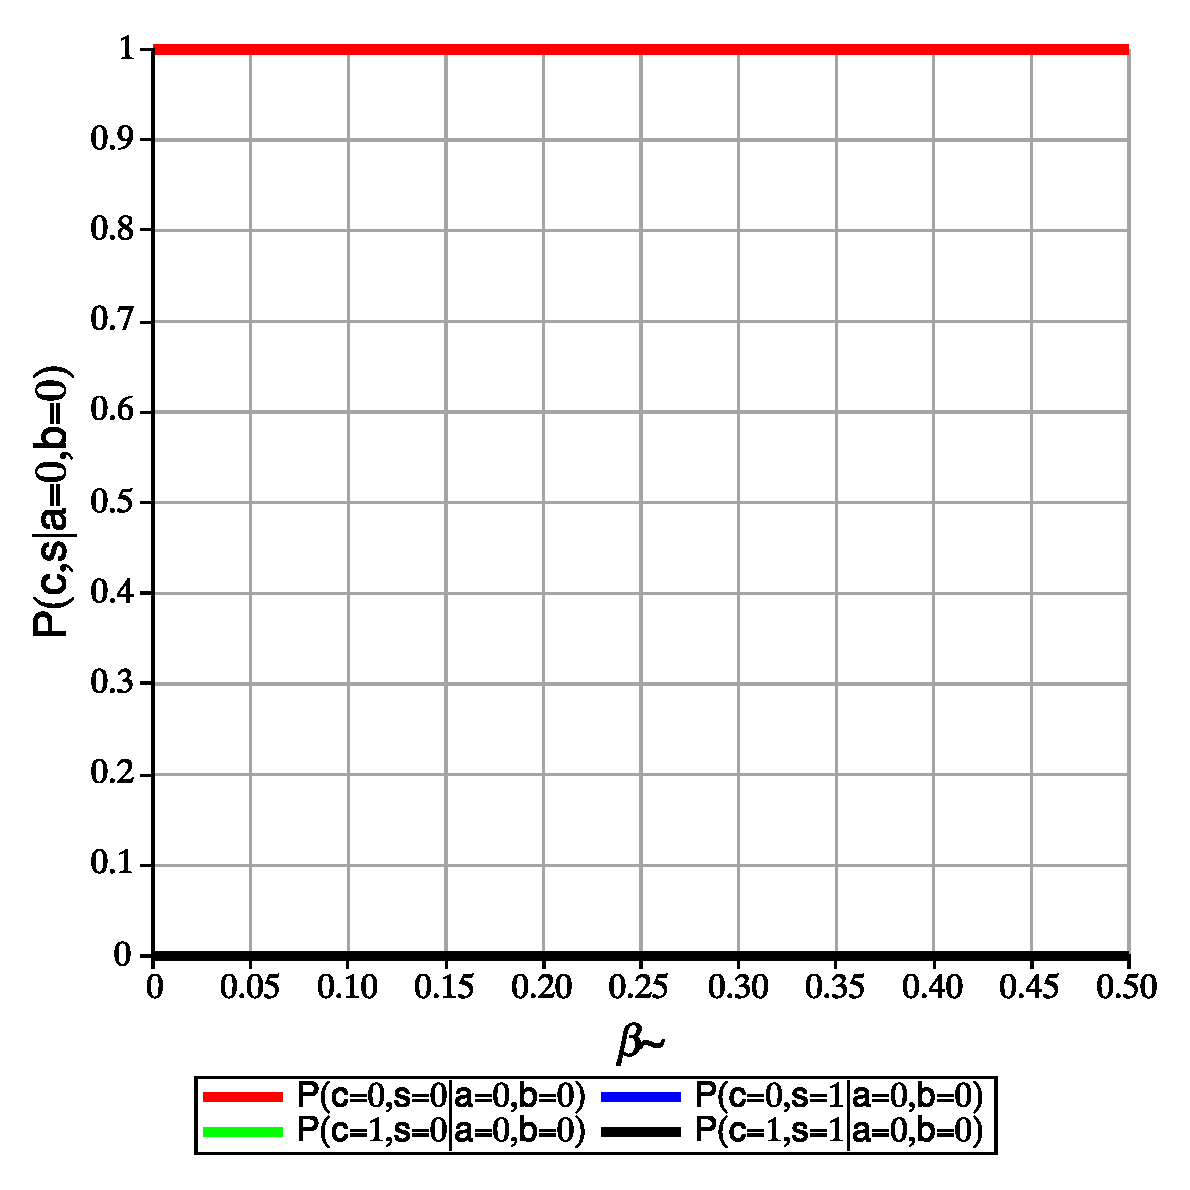
\includegraphics[width=.3\textwidth]{media/noisy_half_adder_value_dist_00.eps} &
        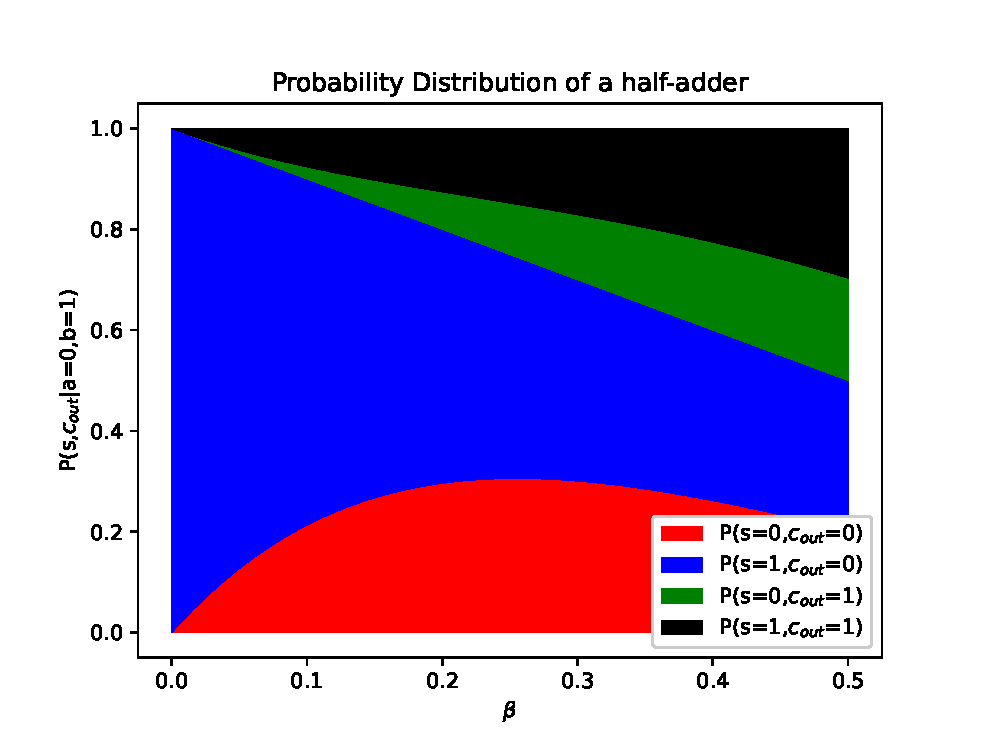
\includegraphics[width=.3\textwidth]{media/noisy_half_adder_value_dist_01.eps} &
        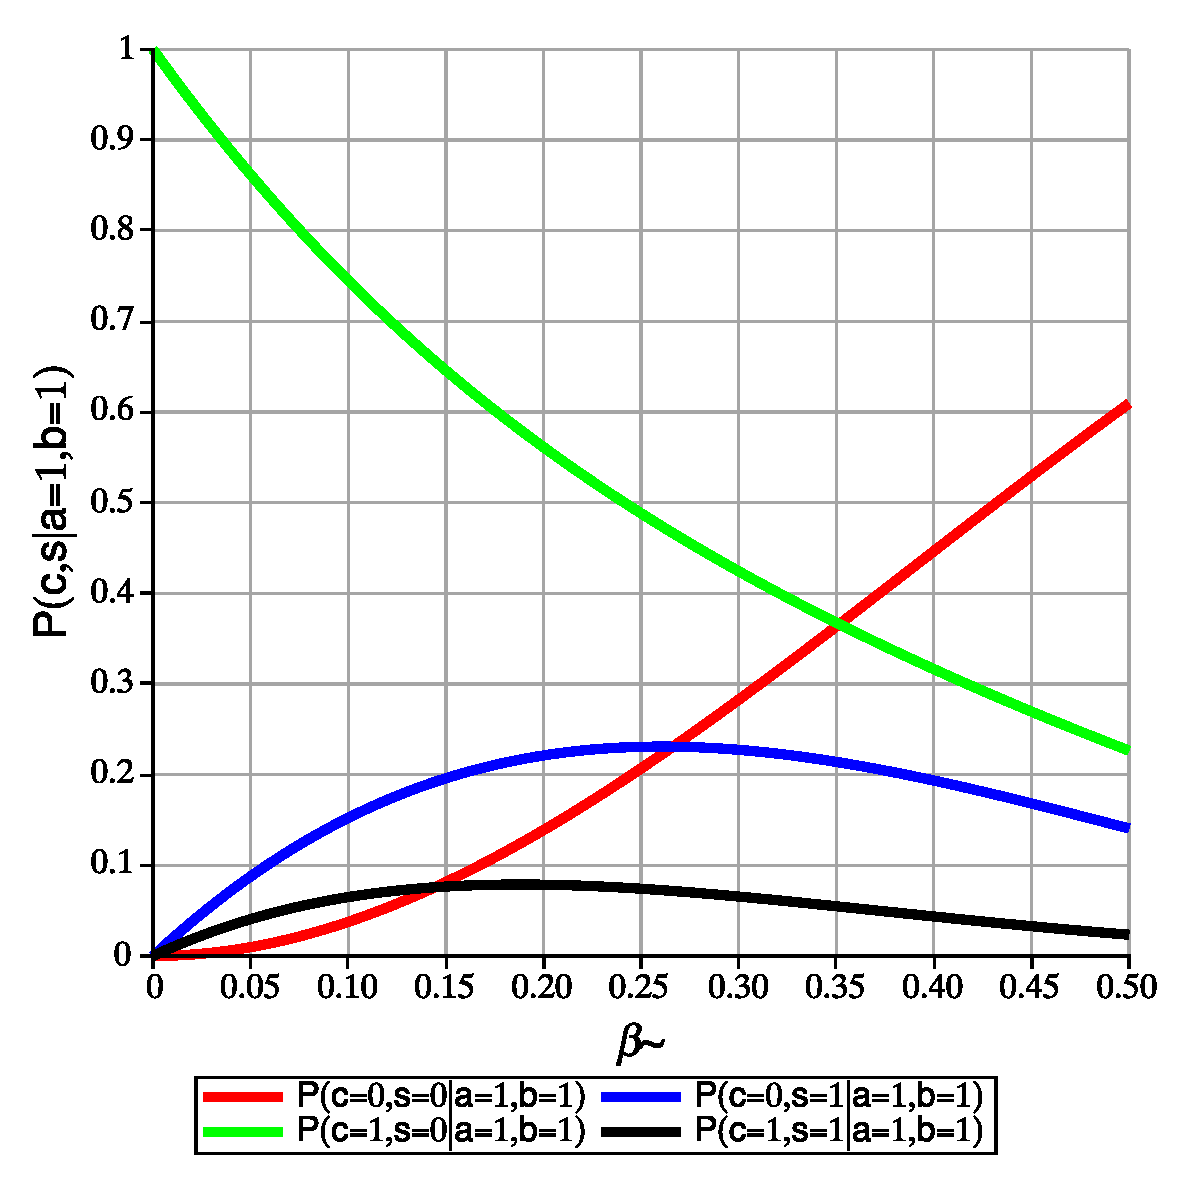
\includegraphics[width=.3\textwidth]{media/noisy_half_adder_value_dist_11.eps} \\
        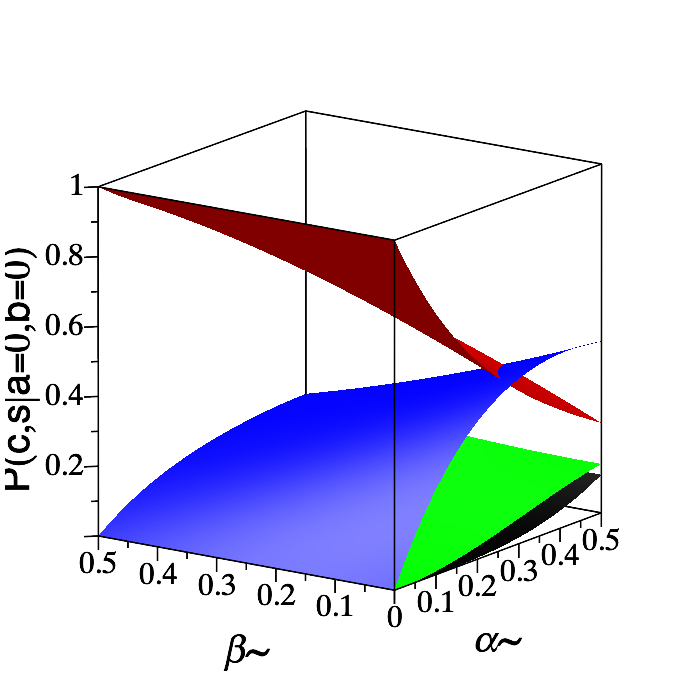
\includegraphics[width=.3\textwidth]{media/noisy_half_adder_value_full_dist_00.png} &
        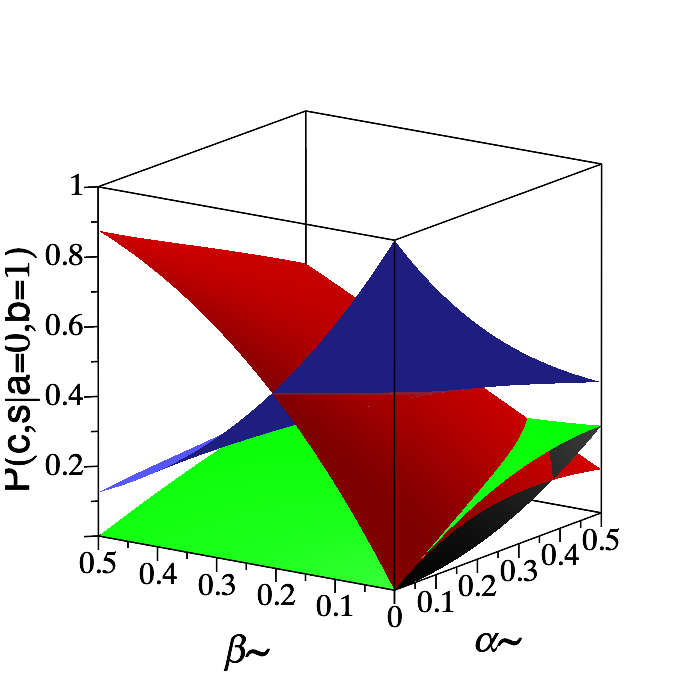
\includegraphics[width=.3\textwidth]{media/noisy_half_adder_value_full_dist_01.png} &
        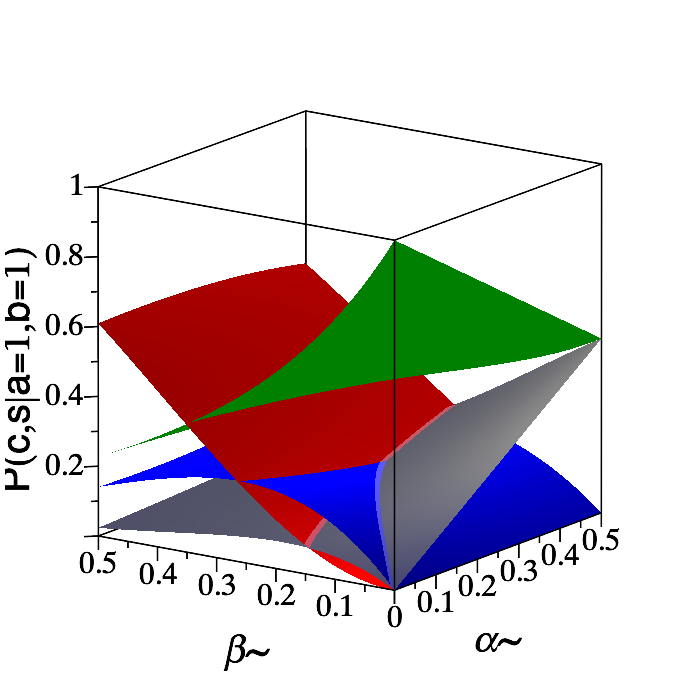
\includegraphics[width=.3\textwidth]{media/noisy_half_adder_value_full_dist_11.png} \\        
    \end{tabular}
    \caption{Probability distribution for $P(s,c|a,b)$ for the three different cases of $a=0, b=0$ (left), $a=0, b=1$ (middle) and $a=1, b=1$ (right), respectively. {\bf Top row:} The graphs show the change of the probability distributions as $\beta$ in (\ref{eq:bit_flip_to_0}) varies from $0$ to $\frac{1}{2}$ and $\alpha = 0$; this case is equivalent to assuming there is only leakage of information due to low-voltage. Note that the errors are not distributed based on the numerical distance of the results, e.g.\ for $\beta=40\%$ the sum of $a=b=1$ is $2$ with probability $\approx 30\%$, $1$ with probability $\approx 20\%$ but $0$ with probability $\approx 45\%$. \label{fig:noise_prob_dist}. {\bf Bottom row:} The 3D graphs show the change of the probability distributions as both $\alpha$ in (\ref{eq:bit_flip_to_1}) and $\beta$ in (\ref{eq:bit_flip_to_0}) varies from $0$ to $\frac{1}{2}$.}
\end{figure}



\begin{figure}
    \centering
    \begin{tikzpicture}
        % Circuit style
        \ctikzset{
            logic ports=ieee,
            logic ports/scale=0.8,
            % logic ports/fill=lightgray
        }

        % Logic ports
        \node[or port] (OR) at (0,0){};
        \node[and port] (ANDa1) at (0,-2){};
        \node[and port] (ANDa2) at (0,-4){};
        \node[or port] (OR2) at (2,-3){};
        \node[not port] (NOT) at (4,-3){};
        \node[and port] (ANDb) at (6,-1.5){};

        % Input and output ports
        \node (a) at (-2,-1) [left] {$a$};
        \node (b) at (-2,-3) [left] {$b$};
        \node (c) at (7,-4) [right] {$c$};
        \node (c1) at (0.8,-2) [above] {$c_1$};
        \node (c2) at (0.8,-4) [above] {$c_2$};
        \node (d) at (1,0) [above] {$d$};
        \node (e) at (4.8,-3) [above] {$e$};
        \node (s) at (7,-1.5) [right] {$s$};
        \node (af) [right = 0.5 of a, coordinate] [left] {};
        \node (bf) [right = 1 of b, coordinate] [left] {};
        \node (cf) at (3,-3) [coordinate] {};

        % % Connection
        \draw (ANDa1.out) -| (OR2.in 1);
        \draw (ANDa2.out) -| (OR2.in 2);
        \draw (OR2.out) -- (NOT.in);
        \draw (OR.out) -| (ANDb.in 1);
        \draw (NOT.out) -| (ANDb.in 2);

        \draw (ANDb.out) -* (s);
        \draw (OR.in 1) -| (af) |- (ANDa1.in 1);
        \draw (OR.in 1) -| (af) |- (ANDa2.in 1);
        \draw (OR.in 2) -| (bf) |- (ANDa2.in 2);
        \draw (OR.in 2) -| (bf) |- (ANDa1.in 2);
        \draw (a) -- (af);
        \draw (b) -- (bf);
        \draw (cf) |- (c);
    \end{tikzpicture}
    \caption{Logic circuit design of a half-adder function with carry-bit redundancy that computes the sum of two binary numbers $a \in \{0,1\}$ and $b \in \{0,1\}$ where $s$ is the sum of $a$ and $b$ and $c$ captures the carry-bit indicating an overflow (i.e., if $a$ and $b$ are both $1$, then $s=0$ and $c=1$). \label{fig:half-adder-fix-carry-bit-redundancy}}
\end{figure}
